\documentclass[border=6pt]{standalone}
\usepackage{amsmath}
\usepackage{amssymb}
\usepackage{tikz}
\usepackage{xcolor}
\usetikzlibrary{arrows.meta,calc,positioning,shapes.geometric}
\begin{document}
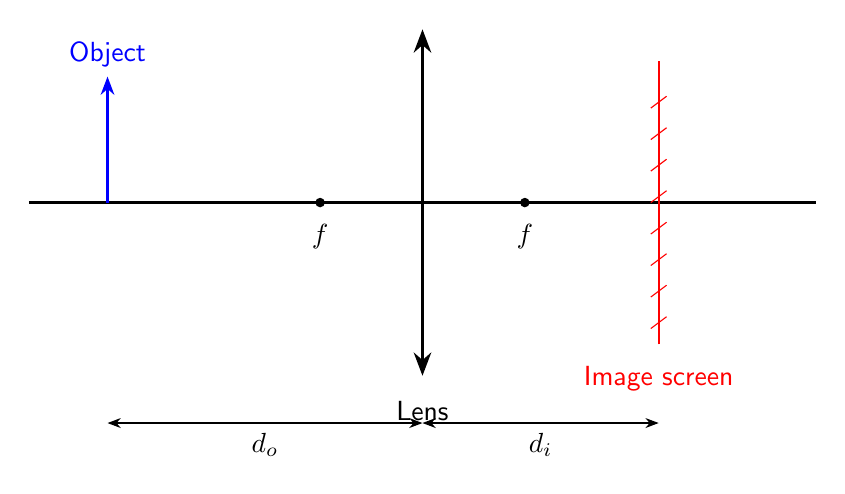
\begin{tikzpicture}[font=\sffamily]
  % optical axis
  \draw[thick] (-5,0) -- (5,0);

  % Lens at x=0: thin-lens symbol (vertical double arrow)
  \draw[very thick, Stealth-Stealth] (0,-2.2) -- (0,2.2);
  \node[below] at (0,-2.4) {Lens};

  % focal points, marked on both sides of the lens
  \filldraw (-1.3,0) circle (1.5pt);
  \node[below] at (-1.3,-0.15) {$f$};
  \filldraw (1.3,0) circle (1.5pt);
  \node[below] at (1.3,-0.15) {$f$};

  % Object: upright arrow, left of the lens
  \draw[-Stealth, thick, blue] (-4,0) -- (-4,1.6);
  \node[above, blue] at (-4,1.6) {Object};

  % Image screen: right of the lens
  \draw[thick, red] (3,-1.8) -- (3,1.8);
  \foreach \y in {-1.6,-1.2,...,1.6} {\draw[red] (2.9,\y) -- (3.1,\y+0.15);}
  \node[below, red] at (3,-1.95) {Image screen};

  % d_o distance marker (Object to Lens)
  \draw[Stealth-Stealth] (-4,-2.8) -- (0,-2.8);
  \node[below] at (-2,-2.8) {$d_o$};

  % d_i distance marker (Lens to Image screen)
  \draw[Stealth-Stealth] (0,-2.8) -- (3,-2.8);
  \node[below] at (1.5,-2.8) {$d_i$};
\end{tikzpicture}
\end{document}
